\documentclass[11pt]{article}
\usepackage[a4paper,margin=21mm]{geometry}
\usepackage{fontspec}
\setmainfont{Latin Modern Roman}
\newfontfamily\CJKfont{Noto Serif CJK SC}
\XeTeXlinebreaklocale "zh"
\XeTeXlinebreakskip=0pt plus 1pt
\usepackage{amsmath,amssymb,amsthm,amscd,graphicx,color}
\usepackage{xurl}
\usepackage[unicode,hidelinks]{hyperref}
\allowdisplaybreaks
\setlength\emergencystretch{3em}
\numberwithin{equation}{section}

\numberwithin{equation}{section}

\newtheorem{Theorem}{Theorem}[section]
\newtheorem{Corollary}[Theorem]{Corollary}
\newtheorem{Lemma}[Theorem]{Lemma}
\newtheorem{Proposition}[Theorem]{Proposition}
{ \theoremstyle{definition}
\newtheorem{Definition}[Theorem]{Definition}
\newtheorem{Note}[Theorem]{Note}
\newtheorem{Example}[Theorem]{Example}
\newtheorem{Remark}[Theorem]{Remark} }

\usepackage{upgreek}
\usepackage[mathscr]{euscript}
\usepackage{cleveref}

\makeatletter\newlabel{fig:qhahn_tasep}{{1}{}{Original source locator}{}{}}\makeatother
\makeatletter\newlabel{thm:intro_qhahn_swap}{{1.1}{}{Original source locator}{}{}}\makeatother
\begin{document}
\begin{center}\Large Local Markov swapping of decreasing neighboring rate parameters in step-initial discrete-time q-Hahn TASEP in the nonnegative-weight regime\end{center}
\noindent\textbf{Stable ID:} 1342\quad\textbf{Author:} Leonid Petrov\par
\noindent\textbf{Work:} Parameter Permutation Symmetry in Particle Systems and Random Polymers\par
\noindent\textbf{Source:} \url{https://sigma-journal.com/2021/021/}\par
\noindent\textbf{Version:} Official SIGMA 17 (2021) article 021, DOI 10.3842/SIGMA.2021.021; journal PDF and native TeX acquired 2026-09-30, exact bytes pinned by SHA256\par
\noindent\textbf{Rights:} CC BY 4.0. Authors retain copyright. \url{https://creativecommons.org/licenses/by/4.0/}. Reuse and typesetting adaptation; original language and mathematical content preserved.\par
\noindent\textbf{Difficulty (prior selection preserved):} {\CJKfont H2: The proof evaluates the swap action on all mixed q-moments and converts its beta-binomial sum into difference operators using the two-body boundary conditions. Acting with those operators inside the nested contour integrals removes exactly one rate and inserts its neighbor, identifying the whole joint law by bounded-moment uniqueness. It then removes the extra contour-separation condition by a finite rational continuation argument and a separate first-particle power-series argument.}\par
\medskip\noindent\textbf{Editorial boundary note (not author text):} Selected complete Theorem3.8 for step-initial discrete-time q-Hahn TASEP at fixed t>=0,0<q<1,nu\_i in(0,1) uniformly bounded below1, and the previously reviewed nonnegative jump regime1<=gamma<1/sup\_i(nu\_i), with nu\_(n+1)<nu\_n. Original broader printed gamma range is preserved literally rather than silently corrected. Exact local transition3.7, configuration/permutation conventions, all beta-binomial/Pochhammer and prior moment formulas, complete contour boundary verification, mixed-moment swap computation and n>=2/n=1 continuation branches are supplied. The temporary contour separation3.5 is explicitly removed by the author, so receives no added conclusion hypothesis. Prior quantum binomial/free-true evolution and published multiparameter moments remain exact background references; no editor extension. Continuous-time/backward/stationary/beta-polymer outcomes are unselected. Original contour asset remains unchanged, with printed labels separately transcribed as editable text; no inference from curves.\par
\noindent\textbf{External original reference fig:qhahn\_tasep:} Original Figure1, native188–193, is a one-step illustration only; exact jump definition3.4 and every nonnegative parameter/formula are retained.\par
\noindent\textbf{External original reference thm:intro\_qhahn\_swap:} Original introductory Theorem1.1, native201–223, states the same swap result; exact complete detailed Theorem3.8 and proof are retained.\par
\medskip\hrule\medskip\noindent\textbf{Author text begins below.}\par
\setcounter{section}{1}
% Original source lines 547--627
\section{From symmetry to swap operators}
\label{sec:general_formalism}

This section contains an abstract discussion of
stochastic particle systems on $\mathbb{Z}$ which
depend symmetrically on their parameters.
The main notions which we use in other parts of the
paper are \emph{parameter-symmetric stochastic particle system}
and \emph{swap operators}.

\subsection{Parameter-symmetric particle systems}
%\label{sub:symm_IPS_def}

Let $\mathrm{Conf}_{\rm fin}(\mathbb{Z})$ be the space of
particle configurations $\mathbf{x}=(\cdots <x_3<x_2<x_1)$,
$x_i\in \mathbb{Z}$,
which can be obtained from the \emph{step configuration}
$\mathsf{step}:=(\ldots,-3,-2,-1 )$
by finitely many operations of moving a particle to the right by one
into the nearby empty spot. The space
$\mathrm{Conf}_{\rm fin}(\mathbb{Z})$ is~countable.

By a multiparameter interacting particle system $\mathbf{x}(t)$
we mean a Markov process on $\mathrm{Conf}_{\rm fin}(\mathbb{Z})$ evolving in continuous
or discrete time,
such that $\mathbf{x}(0)=\mathsf{step}$.
Assume that this Markov process depends on countably many parameters
${\boldsymbol \nu}=\{\nu_i\}_{i\in \mathbb{Z}_{\ge1}}$.
The parameters $\nu_i$ in our situation are real, though without loss of generality
they may belong to an abstract space.
One should think that $\nu_i$ is attached to the particle $x_i$, but the distribution
of each $x_j(t)$ may depend on all of~the~$\nu_i$'s.
We denote the process depending on ${\boldsymbol \nu}$ by $\mathbf{x}^{{\boldsymbol \nu}}(t)$.
In this section we assume that all the parameters $\nu_i$ are pairwise distinct.

The infinite symmetric group
$S(\infty)=\bigcup_{n=1}^{\infty}S(n)$
acts on the parameters ${\boldsymbol \nu}$ by permutations,
$\sigma\colon {\boldsymbol \nu}\mapsto \sigma{\boldsymbol \nu}$.
Here $S(n)$ is the symmetric group which permutes only the
first parame\-ters~$\nu_1,\ldots,\nu_n$.
Let us denote by $S_n(\infty)\subset S(\infty)$
the subgroup which permutes $\nu_{n+1},\nu_{n+2},\ldots $
and maps each $\nu_i$, $1\le i\le n$, into itself. Note that
$S(n)\cap S_n(\infty)=S(n)\cap S_{n-1}(\infty)=\{e\}$,
and~$S(n+1)\cap S_{n-1}(\infty)=\{e,s_{n}\}$,
where $e$ is the identity permutation, and
$s_{n}=(n,n+1)$ is the transposition
$n\leftrightarrow n+1$.

By imposing a specific distributional symmetry
of $\mathbf{x}^{{\boldsymbol \nu}}(t)$
under the action of $S(\infty)$
on the parameters ${\boldsymbol \nu}$, we arrive at the following definition:

\begin{Definition}
	\label{def:symm_IPS}
	A multiparameter particle system $\mathbf{x}^{{\boldsymbol \nu}}(t)$ is called \emph{parameter-symmetric},
	if for all $n$ and $t$ we have
	the following equality of joint distributions:
\begin{gather}
\big(\ldots,x_{n+2}^{{\boldsymbol \nu}}(t),x_{n+1}^{{\boldsymbol \nu}}(t),
x_{n-1}^{{\boldsymbol \nu}}(t),\ldots, x_1^{{\boldsymbol \nu}}(t)\big)\nonumber
\\ \qquad
{}\stackrel{d}{=}\big(\ldots,x_{n+2}^{s_n{\boldsymbol \nu}}(t),x_{n+1}^{s_n{\boldsymbol \nu}}(t),
x_{n-1}^{s_n{\boldsymbol \nu}}(t),\ldots,x_1^{s_n{\boldsymbol \nu}}(t)\big).
\label{eq:symm_IPS}
\end{gather}
	That is, the transposition $s_n$ preserves the joint
	distribution of all particles except $x_n$.
\end{Definition}
Here is a straightforward corollary of this definition:
\begin{Corollary}
	In a parameter-symmetric particle system,
	for any $t$ and any $\sigma\in S(n)\cup S_{n}(\infty)$, the
	random variables
	$x_n^{{\boldsymbol \nu}}(t)$ and
	$x_n^{\sigma {\boldsymbol \nu}}(t)$
	have the same distribution.
\end{Corollary}


\setcounter{section}{2}\setcounter{footnote}{3}\setcounter{figure}{2}
% Original source lines 816--1345
\section[Swap operators for q-Hahn TASEP]{Swap operators for $\boldsymbol q$-Hahn TASEP}\label{sec:qhahn_TASEP}

{\sloppy
In this section we examine the parameter symmetry and swap operators for the
$q$-Hahn TASEP~\cite{Povolotsky2013}.
A multiparameter version of the process
preserving its integrability is due to~\cite{BorodinPetrov2016inhom}.

}

\subsection[The q-deformed beta-binomial distribution]
{The $\boldsymbol q$-deformed beta-binomial distribution}\label{sub:phi_distribution}

We first recall the definition and properties of
the $q$-deformed beta-binomial distribution
$\varphi_{q,\mu,\nu}$ from~\cite{Corwin2014qmunu, Povolotsky2013}.
We use the standard notation for the $q$-Pochhammer symbol
$(x;q)_k=(1-x)\times(1-qx)\cdots\big(1-q^{k-1}x\big)$, $k\in \mathbb{Z}_{\ge1}$
(by agreement, $(x;q)_0=1$).

Everywhere throughout the paper we
assume that the main parameter $q$ is between $0$ and $1$.

\begin{Definition}
	\label{def:phi_distribution}
	For $m\in \mathbb{Z}_{\ge0}$, consider the following distribution on
	$\left\{ 0,1,\ldots,m \right\}$:
	\begin{gather*}
		\varphi_{q,\mu,\nu}(j\,|\, m)=
		\mu^j\,\frac{(\nu/\mu;q)_j(\mu;q)_{m-j}}{(\nu;q)_m}
		\frac{(q;q)_m}{(q;q)_j(q;q)_{m-j}},
		\qquad
		0\le j\le m.
	\end{gather*}
	When $m=+\infty$, extend the definition as
	\begin{gather*}
		\varphi_{q,\mu,\nu}(j\,|\, \infty)=
		\mu^j\frac{(\nu/\mu;q)_j}{(q;q)_j}\frac{(\mu;q)_\infty}{(\nu;q)_\infty},
		\qquad
		j\in \mathbb{Z}_{\ge0}.
	\end{gather*}
	The distribution depends on $q$
	and two other parameters~$\mu,\nu$.
\end{Definition}

When $0\le \mu\le 1$ and $\nu\le \mu$, the weights $\varphi_{q,\mu,\nu}(j\,|\, m)$
are nonnegative.\footnote{These conditions do not
exhaust the full range of $(q,\mu,\nu)$
for which the weights are nonnegative.
See, e.g., \cite[Section 6.6.1]{BorodinPetrov2016inhom}
for additional families of parameters leading to nonnegative weights.}
They also sum to~one:
\begin{gather*}
\sum_{j=0}^{m}\varphi_{q,\mu,\nu}(j\,|\, m)=1,\qquad m\in\{ 0,1,\ldots \}
\cup\{ +\infty \}.
\end{gather*}
We will need two other properties of the weights given in the next
two lemmas.

\begin{Lemma}[\cite{Barraquand_qhahn_2014, Corwin2014qmunu}]
	\label{lemma:phi_symmetry}
	The weights satisfy a symmetry property: for all
	$m,y\in \mathbb{Z}_{\ge0}$ we have
	\begin{gather*}
		\sum_{j=0}^{m}q^{jy}\varphi_{q,\mu,\nu}(j\,|\, m)
		=\sum_{k=0}^{y} q^{km}\varphi_{q,\mu,\nu}(k\,|\, y).
	\end{gather*}
	Similarly, for all $y\in \mathbb{Z}_{\ge0}$, we have
	\begin{gather*}
		\sum_{j=0}^{\infty}q^{jy}\varphi_{q,\mu,\nu}(j\,|\, \infty)=
		\varphi_{q,\mu,\nu}(0\,|\, y).
	\end{gather*}
\end{Lemma}

Define the following difference operator:
\begin{gather}
	\label{eq:nabla_mu_nu}
	(\nabla_{\mu,\nu}f)(n):=\frac{\mu-\nu}{1-\nu}\,f(n-1)+\frac{1-\mu}{1-\nu}\,f(n).
\end{gather}

The next statement is a key property of the $q$-deformed beta binomial distribution
which allows to simplify the action of certain operators defined through $\varphi_{q,\mu,\nu}$
on functions satisfying special boundary conditions. This is a manifestation of the
connection of $\varphi_{q,\mu,\nu}$ to the coordinate Bethe ansatz, as
developed in~\cite{Povolotsky2013}.
\begin{Lemma}
	\label{lemma:phi_duality}
	Fix parameters $\nu_i\in(0,1)$, $i\in \mathbb{Z}$.
	Let a function $f(n_1,\ldots,n_m )$ from
	$\mathbb{Z}^{m}$ to $\mathbb{C}$ satisfy the following
	two-body
	boundary conditions
\begin{gather}
\frac{\nu_{n_i}(1-q)}{1-q\nu_{n_i}}\,f(n_1,\ldots,n_{i}-1,n_{i+1}-1,\ldots ,n_m)
+\frac{q-\nu_{n_i}}{1-q\nu_{n_i}}\,f(n_1,\ldots,n_i,n_{i+1}-1,\ldots ,n_m)\nonumber
\\ \qquad
{}	+\frac{1-q}{1-q\nu_{n_i}}\,f(n_1,\ldots,n_i,n_{i+1},\ldots ,n_m)
-f(n_1,\ldots,n_i-1,n_{i+1},\ldots ,n_m)=0
		\label{eq:q_hahn_boundary_conditions}
		\end{gather}
	for all $\vec n\in \mathbb{Z}^m$
	such that for some $i \in \left\{ 1,\ldots,m \right\}$,
	$n_i=n_{i+1}$. $($In~\eqref{eq:q_hahn_boundary_conditions},
	only the $i$-th and the $(i+1)$-st components of $\vec n$
	are changed.$)$ Then we have
	\begin{gather}
		\label{eq:quantum_binomial_variable}
		\prod_{i=1}^{m}[\nabla_{\mu,\nu_{n}}]_i \,
		f(\underbrace{n,n,\ldots,n}_m)
		=
		\sum_{j=0}^{m}
		\varphi_{q,\mu,\nu_{n}}(j\,|\, m)\,
		f(\underbrace{n,\ldots,n }_{m-j},\underbrace{n-1,\ldots,n-1 }_{j}).
	\end{gather}
	Here $[\nabla_{\mu,\nu_{n}}]_i$ is the operator~\eqref{eq:nabla_mu_nu}
	applied in the $i$-th variable.
\end{Lemma}
\begin{proof}
	This is based on the quantum (noncommutative) binomial
	\cite[Theorem 1]{Povolotsky2013}, and is a~straightforward generalization of the
	equivalence of the free and true evolution equations
	\cite[Proposition 1.8]{Corwin2014qmunu}.
	The only difference here is that $\nu_i$'s are allowed to vary.
	However, as the application of the quantum binomial
	result depends only on the parameter $\nu_n$ associated
	to the particular $n$ in~\eqref{eq:quantum_binomial_variable},
	we see that the claim readily holds.
\end{proof}


\subsection[Multiparameter q-Hahn TASEP]
{Multiparameter $\boldsymbol q$-Hahn TASEP}\label{sub:qhahn_defn}

Here we recall the particle-inhomogeneous version of
the $q$-Hahn TASEP from \cite[Section 6.6]{BorodinPetrov2016inhom}.
Let
\begin{gather*}
	\nu_i\in(0,1),\qquad i\in \mathbb{Z}_{\ge1},\qquad
	\gamma\in\bigl[1,\sup\nolimits_{i}\nu_i^{-1}\bigr]
\end{gather*}
be parameters.
To make the system nontrivial, the $\nu_i$'s should be uniformly
bounded away from~$1$.


The $q$-Hahn TASEP starts from $\mathsf{step}$ and
evolves in
$\mathrm{Conf}_{\rm fin}(\mathbb{Z})$
in discrete time $t\in \mathbb{Z}_{\ge0}$.
At~each time moment, each particle $x_i$ independently
jumps to the right by $j$ with probability
\begin{gather}
	\label{eq:qhahn_one_step_jump}
	\varphi_{q,\gamma\nu_i,\nu_i}(j\,|\, x_{i-1}-x_i-1),
	\qquad
	j\in \left\{ 0,1,\ldots,x_{i-1}-x_i-1 \right\},
\end{gather}
where $x_0=+\infty$, by agreement.
See Fig.~\ref{fig:qhahn_tasep} for an illustration.
For the step initial configuration
the $q$-moments of the $q$-Hahn TASEP were
obtained in \cite[Corollary 10.4]{BorodinPetrov2016inhom}
(in the homogeneous case $\nu_i\equiv \nu$
a proof using duality and coordinate
Bethe ansatz
is due to
\cite{Corwin2014qmunu}). The $q$-moments are given in the next proposition.
\begin{Proposition}
	%\label{prop:q_hahn_q_moments}
	For any $\ell\in \mathbb{Z}_{\ge1}$
	and any $n_1\ge n_2\ge \dots\ge n_\ell\ge1$
	with the assumption that
	\begin{gather}
		\label{eq:qhahn_nu_contour_existence_assumption}
		\min_{1\le i\le n_1}
		\nu_i>q \max_{1\le i\le n_1} \nu_i
	\end{gather}
	we have for the $q$-moments of the $q$-Hahn TASEP started from $\mathsf{step}$:
	\begin{gather}
\mathbb{E}^{\mathrm{qH}(\boldsymbol\nu)}_{\mathsf{step}}
\prod_{j=1}^{\ell}q^{x_{n_j}(t)+n_j}= 
			(-1)^{\ell}q^{\frac{\ell(\ell-1)}{2}}
			\oint\frac{{\rm d}z_1}{2\pi\mathbf{i}}
			\cdots
			\oint\frac{{\rm d}z_\ell}{2\pi\mathbf{i}}
			\prod_{1\le A<B\le \ell}\frac{z_A-z_B}{z_A-qz_B}\nonumber
\\ \hphantom{\mathbb{E}^{\mathrm{qH}(\boldsymbol\nu)}_{\mathsf{step}}
\prod_{j=1}^{\ell}q^{x_{n_j}(t)+n_j}= }
{}\times\prod_{i=1}^{\ell}\left(\bigg( \frac{1-\gamma z_i}{1-z_i} \bigg)^t
\frac{1}{z_i(1-z_i)}\prod_{j=1}^{n_i}\frac{1-z_i}{1-z_i/\nu_j} \right).
\label{eq:qhahn_step_moments}
\end{gather}
	Here the integration contours are positively oriented simple
	closed curves which are
	$q$-nested around $\{\nu_j\}_{j=1,\ldots,n_1 }$
	$($that is, each contour encircles the $\nu_j$'s, and, moreover, the $z_A$ contour
	encircles each $qz_B$ contour, $B>A)$
	and leave $0$ and $1$ outside. See
	Fig.~$\ref{fig:qhahn_contours}$ for an illustration.
\end{Proposition}

\begin{figure}[htpb]
	\centering
	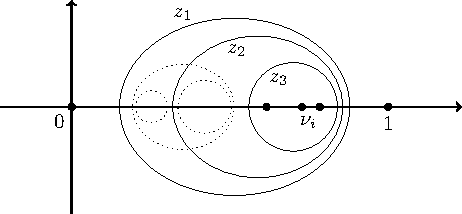
\includegraphics[scale=1.1]{../assets/1342/fig-qhahn-step-contours.pdf}
	\caption{Possible integration contours in~\eqref{eq:qhahn_step_moments}
	for $\ell=3$. The contours for $qz_3$, $q^2z_3$, and $qz_2$ are shown dotted.}
	\label{fig:qhahn_contours}
\end{figure}

\begin{Remark}
	\label{rmk:inhom_time}
	Together with particle-dependent inhomogeneity governed by
	the parameters $\nu_i$, one can make the parameter $\gamma$ time-dependent.
	That is, at each time step $t-1\to t$, the jumping distribution
	\eqref{eq:qhahn_one_step_jump} can be replaced by
	$\varphi_{q,\gamma_t\nu_i,\nu_i}(j\,|\, x_{i-1}-x_i-1)$.
	The moment formula~\eqref{eq:qhahn_step_moments} continues to hold
	when modified by replacing the term $\bigl( \frac{1-\gamma z_i}{1-z_i} \bigr)^t$
	with
	$\prod_{l=1}^t\frac{1-\gamma_l z_i}{1-z_i}$. The main result
	of this section (Theorem~\ref{thm:qhahn_swap} below)
	also holds in this generality,
	but for simplicity we will continue to assume that $\gamma$
	does not depend on $t$.
\end{Remark}

Since $0<q<1$ and we start from $\mathsf{step}$, the random variables
$\prod_{j=1}^{\ell}q^{x_{n_j}(t)+n_j}$ are all between~$0$ and~$1$.
Because the moment problem
for bounded random variables admits a unique solution,
the $q$-moments~\eqref{eq:qhahn_step_moments}
uniquely determine the joint distribution of
all the
$q$-Hahn TASEP particles $\{x_i(t)\}_{i\in \mathbb{Z}_{\ge1}}$ at each fixed time moment.
This implies the following statement:

\begin{Proposition}
	%\label{prop:q_hahn_step_symmetry}
	The multiparameter $q$-Hahn TASEP
	started from the step initial configuration
	is a parameter-symmetric particle system in the sense of
	Definition~$\ref{def:symm_IPS}$.
	Moreover, the distribution of each $x_n(t)$
	depends on the parameters $\nu_1,\ldots,\nu_n $ in a symmetric way.
\end{Proposition}

Denote the right-hand of~\eqref{eq:qhahn_step_moments}
by $f(n_1,\ldots,n_\ell )$, where now $n_i\in \mathbb{Z}$ are not necessarily ordered.
Notice that if $n_\ell=0$, the integrand has no poles inside the $z_\ell$ (i.e., the smallest)
integration contour.
Therefore,
$f(n_1,\ldots,n_{\ell-1},0 )=0$.
The following lemma will be employed in the next section.

\begin{Lemma}
	\label{lemma:boundary_conditions}
	The function $f(n_1,\ldots,n_\ell )$ on $\mathbb{Z}^{\ell}$ defined before the lemma
	satisfies the two-body boundary conditions
	\eqref{eq:q_hahn_boundary_conditions}.
\end{Lemma}
\begin{proof}
	This statement essentially appears in
	\cite{Corwin2014qmunu}, see also~\cite{BorodinCorwinSasamoto2012}.
	Its proof is rather short so we reproduce it here.
	When $n_i=n_{i+1}$ (denote them both by $n$),
	the part of the integrand in~\eqref{eq:qhahn_step_moments} depending on
	$z_i$, $z_{i+1}$ contains
	\begin{gather*}
		\frac{z_i-z_{i+1}}{z_i-qz_{i+1}}
		\prod_{j=1}^{n}\frac{(1-z_i)(1-z_{i+1})}{(1-z_i/\nu_j)(1-z_{i+1}/\nu_j)}.
	\end{gather*}
	The left-hand side of the boundary conditions
	\eqref{eq:q_hahn_boundary_conditions} for our function $f$
	is an integral over the contours as in Fig.~\ref{fig:qhahn_contours}, where the integrand now contains
	\begin{gather*}
	\frac{z_i-z_{i+1}}{z_i-qz_{i+1}}
	\prod_{j=1}^{n-1}\frac{(1-z_i)(1-z_{i+1})}{(1-z_i/\nu_j)(1-z_{i+1}/\nu_j)}
	\\ \hphantom{\frac{z_i-z_{i+1}}{z_i-qz_{i+1}}}
	{}\times
	\bigg(\frac{\nu_n(1\!-\!q)}{1\!-\!q \nu_n}+\frac{q\!-\!\nu_n}{1\!-\!q \nu_n}\frac{1\!-\!z_i}{1\!-\!z_i/\nu_n}
	+\frac{1\!-\!q}{1\!-\!q \nu_n}\frac{1\!-\!z_i}{1\!-\!z_i/\nu_n}\frac{1\!-\!z_{i+1}}{1\!-\!z_{i+1}/\nu_n}
	-\frac{1\!-\!z_{i+1}}{1\!-\!z_{i+1}/\nu_n}\bigg)
	\\ \hphantom{\frac{z_i-z_{i+1}}{z_i-qz_{i+1}}}
{}=\frac{\nu_n(1-\nu_n)^2}{1-q\nu_n}
	\frac{z_i-z_{i+1}}{(z_i-\nu_n)(z_{i+1}-\nu_n)}
	\prod_{j=1}^{n-1}\frac{(1-z_i)(1-z_{i+1})}{(1-z_i/\nu_j)(1-z_{i+1}/\nu_j)},
	\end{gather*}
	where the important observation is that
	the denominator $z_i-qz_{i+1}$ has
	canceled out. Now the contour for $z_{i}$ can be deformed
	(without picking any residues) to coincide with the contour for $z_{i+1}$.
	However, thanks to the factor $z_i-z_{i+1}$, the integrand is antisymmetric in
	$z_i$, $z_{i+1}$. Therefore, the whole integral vanishes, as desired.
\end{proof}

\subsection[Markov swap operators for q-Hahn TASEP]
{Markov swap operators for $\boldsymbol q$-Hahn TASEP}
\label{sub:cond_distr_qhahn}

Here we prove that the $q$-Hahn TASEP
admits a local conditional distribution
corresponding to the permutation $s_n=(n,n+1)$
when the parameters satisfy $\nu_{n+1}<\nu_n$ before their swap.
This leads to the Markov swap operator which we define now.
Fix $n\in \mathbb{Z}_{\ge1}$,
and let
\begin{gather}
	\label{eq:qhahn_transition_prob}
	p_n^{\mathrm{qH}}
	(x_n'\,|\, x_{n+1},x_n,x_{n-1}):=
	\varphi_{q,\frac{\nu_{n+1}}{\nu_n},\nu_{n+1}}(x_n'-x_{n+1}-1\,|\, x_n-x_{n+1}-1).
\end{gather}
Observe that this probability does not depend on $x_{n-1}$.
The condition $\nu_{n+1}<\nu_n$ ensures that
the swap operator $p_n^{\mathrm{qH}}$
\eqref{eq:qhahn_transition_prob}
has nonnegative probability weights.
\begin{Theorem}[Theorem~\ref{thm:intro_qhahn_swap} in Introduction]
	\label{thm:qhahn_swap}
	Let $\mathbf{x}^{\boldsymbol\nu}(t)$ be the $q$-Hahn TASEP with parameters
	$\boldsymbol\nu=\{\nu_i\}_{i\in \mathbb{Z}_{\ge1}}$,
	started from $\mathsf{step}$.
	Fix $n\in \mathbb{Z}_{\ge1}$ and assume that
	$\nu_{n+1}<\nu_n$.
	Replace $x_n(t)$ by a~random $x_n'(t)$ coming from the Markov swap operator
	$p_n^{\mathrm{qH}}$~\eqref{eq:qhahn_transition_prob}.
	Then the new configuration is distributed as the $q$-Hahn TASEP $\mathbf{x}^{s_n \boldsymbol\nu}(t)$
	with swapped parameters.
\end{Theorem}
\begin{proof}
	We will prove this theorem by applying
	$p_n^{\mathrm{qH}}$
	in the $q$-moment formula.
	Since the $q$-mo\-ments uniquely determine
	the distribution, this computation will imply the claim.
	
	Fix integers $\ell,\ell',a,b\ge0$ and define
	\begin{gather}
	\label{eq:n_a_b_notation}
	\vec n=(n_1,\ldots,n_k ):=(m_1,\ldots,m_\ell,\underbrace{n+1,\ldots,n+1 }_a,
 \underbrace{n,\ldots,n }_b,m_1',\ldots,m'_{\ell'}),
	\end{gather}
	where $m_1\ge \dots\ge m_\ell>n+1$,
	$n>m_1'\ge \dots\ge m'_{\ell'}\ge1$, and
	$k=\ell+a+b+\ell'$.
	Assume that the parameters $\nu_i$ satisfy
	the contour existence condition
	\eqref{eq:qhahn_nu_contour_existence_assumption}. (In the end
	of the proof we will drop this assumption.)
	It suffices to show that
	\begin{gather}
		\label{eq:expectation_Markov_chain_action}
		\mathbb{E}^{\mathrm{qH}(\boldsymbol\nu)}_{\mathsf{step}}
		\bigg(
			\sum_{x_n'=x_{n+1}(t)+1}^{x_n(t)}
			p_n^{\mathrm{qH}}
			(x_n'\,|\, x_{n+1}(t),x_n(t),x_{n-1}(t))
			\,q^{b(x_n'+n)}
			\prod_{\substack{j=1 \\n_j\ne n}}^{k}q^{x_{n_j}(t)+n_j}
		\biggr)
	\end{gather}
	(where the expectation
	$\mathbb{E}^{\mathrm{qH}(\boldsymbol\nu)}_{\mathsf{step}}$
	is taken with the
	parameters before the swap),
	is equal to the expectation
	\begin{gather}
		\label{eq:expectation_desired_for_qhahn}
		\mathbb{E}^{\mathrm{qH}(s_n\boldsymbol\nu)}_{\mathsf{step}}
		\prod_{j=1}^{k}q^{x_{n_j}(t)+n_j}
	\end{gather}
	with the swapped parameters.
	Indeed,
	the sum over $x_n'$
	in
	\eqref{eq:expectation_Markov_chain_action}
	corresponds to the action of the swap operator
	$p_n^{\mathrm{qH}}$
	on
	$\prod_{j=1}^{k}q^{x_{n_j}(t)+n_j}$ viewed as a function of $\{x_i(t)\}$.
	We thus need to show that the expectation of the result
	with respect to the original parameters
	leads to
	the formula with the swapped parameters.
	
	
	
	We now start from~\eqref{eq:expectation_Markov_chain_action}, and
	in the rest of the proof omit the dependence on $t$ for shorter notation.
	First, we use the symmetry property (Lemma~\ref{lemma:phi_symmetry})
	to write for the part of the sum in~\eqref{eq:expectation_Markov_chain_action}
	involving $x_n$, $x_{n+1}$:
	\begin{gather}
	\sum_{x_n'=x_{n+1}+1}^{x_n}
	\varphi_{q,\frac{\nu_{n+1}}{\nu_n},\nu_{n+1}}(x_n'-x_{n+1}-1\,|\, x_n-x_{n+1}-1)
	\,q^{a(x_{n+1}+n+1)+b(x_n'+n)}\nonumber
	\\[-.5ex] \qquad
{}=	\sum_{x_n'=x_{n+1}+1}^{x_n}	\!\!\! q^{b(x_n'-x_{n+1}-1)}
	\varphi_{q,\frac{\nu_{n+1}}{\nu_n},\nu_{n+1}}
	(x_n'-x_{n+1}-1\,|\, x_n-x_{n+1}-1)	\,q^{(a+b)(x_{n+1}+n+1)}\nonumber
	\\[-.5ex] \qquad
{}=	\sum_{r=0}^{b}	q^{r(x_n-x_{n+1}-1)}	\varphi_{q,\frac{\nu_{n+1}}{\nu_n},\nu_{n+1}}
	(r\,|\, b)	\,q^{(a+b)(x_{n+1}+n+1)}\nonumber
	\\[-.5ex] \qquad
{}=	\sum_{r=0}^{b}	\varphi_{q,\frac{\nu_{n+1}}{\nu_n},\nu_{n+1}}
	(r\,|\, b)	\,q^{(a+b-r)(x_{n+1}+n+1)+r(x_n+n)}.
	\label{eq:duality_computation_for_ptransition}
	\end{gather}

	We thus need to compute
	\begin{gather}
		\label{eq:thm_qhahn_swap_proof1}
		\sum_{r=0}^{b}
		\varphi_{q,\frac{\nu_{n+1}}{\nu_n},\nu_{n+1}}
		(r\,|\, b)
		\,\mathbb{E}^{\mathrm{qH}(\boldsymbol\nu)}_{\mathsf{step}}
		\biggl(\prod_{j=1}^{k}
		q^{x_{n_j(r)}+n_j(r)}\biggr),
	\end{gather}
	where the vector
	$\vec n(r)=(n_1(r),\ldots,n_k(r) )$
	is as in~\eqref{eq:n_a_b_notation},
	but with $(a,b)$ replaced by $(a+b-r,r)$.
	The expectation in~\eqref{eq:thm_qhahn_swap_proof1}
	is given by the contour integral as in the right-hand side of
	\eqref{eq:qhahn_step_moments}.
	Recall the notation $f(\vec n)$ for this integral, where now $\vec n\in \mathbb{Z}^k$,
	and the components of $\vec n$ are not necessarily ordered.
	By Lemma~\ref{lemma:boundary_conditions}, this function $f$ satisfies the two-body boundary conditions.
	Thus,~\eqref{eq:thm_qhahn_swap_proof1} can be rewritten by Lemma~\ref{lemma:phi_duality}
	as (recall notation~\eqref{eq:nabla_mu_nu} for
	the operator
	$\nabla_{\mu,\nu}$):
	\begin{gather*}
		\prod_{j=1}^{b}\left[ \nabla_{\frac{\nu_{n+1}}{\nu_n},\nu_{n+1}} \right]_{\ell+a+j}\,
		f(m_1,\ldots,m_\ell,\underbrace{n+1,\ldots,n+1 }_{a+b},m_1',\ldots,m'_{\ell'}).
	\end{gather*}
	Observe that now
	each of the difference operators
	$[ \nabla_{\frac{\nu_{n+1}}{\nu_n},\nu_{n+1}} ]_{\ell+a+j}$
	can be applied independently
	inside the integral. We thus have for every variable $w=z_{\ell+a+j}$,
	$j=1,\ldots,b $:
	\begin{gather*}
	[\nabla_{\frac{\nu_{n+1}}{\nu_n},\nu_{n+1}}]_{\ell+a+j}
	\prod_{i=1}^{n+1}\frac{1\!-\!w}{1\!-\!w/\nu_i}
	=	\bigg( \frac{\nu_{n+1}/\nu_n\!-\!\nu_{n+1}}{1\!-\!\nu_{n+1}}+
	\frac{1\!-\!\nu_{n+1}/\nu_n}{1\!-\!\nu_{n+1}}\frac{1\!-\!w}{1\!-\!w/\nu_{n+1}} \bigg)
	\prod_{i=1}^{n}\frac{1\!-\!w}{1\!-\!w/\nu_i}
	\\ \hphantom{[\nabla_{\frac{\nu_{n+1}}{\nu_n},\nu_{n+1}}]_{\ell+a+j}
	\prod_{i=1}^{n+1}\frac{1\!-\!w}{1\!-\!w/\nu_i}}
{}=	\frac{1-w/\nu_n}{1-w/\nu_{n+1}}	\prod_{i=1}^{n}\frac{1-w}{1-w/\nu_i}
	=\prod_{\substack{i=1\\i\ne n}}^{n+1}\frac{1-w}{1-w/\nu_i}.
	\end{gather*}
	We see that the
	resulting integral coming from~\eqref{eq:expectation_Markov_chain_action}
	contains, for each variable
	$z_{\ell+a+j}$ corresponding to $n_{\ell+a+j}=n$ in~\eqref{eq:n_a_b_notation}, the product over the
	parameters $(\nu_1,\ldots,\nu_{n-1},\nu_{n+1} )=s_n(\nu_1,\ldots,\nu_{n} )$.
	Therefore, this integral is equal to the
	expectation~\eqref{eq:expectation_desired_for_qhahn}
	with the swapped parameters $s_n\boldsymbol\nu$, as desired.

	

	It remains to show that we can drop the contour
	existence assumption~\eqref{eq:qhahn_nu_contour_existence_assumption}.
	The preceding argument implies that
	under~\eqref{eq:qhahn_nu_contour_existence_assumption} (with fixed $x_{n+1},x_n',x_{n-1}$),
	\begin{gather}
		\sum_{x_n=x_n'}^{x_{n-1}-1}
		P_{\boldsymbol\nu}(\ldots,x_{n+1},x_n,x_{n-1},\ldots )\,
		\varphi_{q,\frac{\nu_{n+1}}{\nu_n},\nu_{n+1}}(x_n'-x_{n+1}-1\,|\, x_n-x_{n+1}-1)\nonumber
		\\ \qquad
{}=		P_{s_n\boldsymbol\nu}(\ldots, x_{n+1},x_{n}',x_{n-1},\ldots ),
		\label{eq:analytic_continuation}
	\end{gather}
	where $P_{\boldsymbol\nu}$, $P_{s_n\boldsymbol\nu}$ denote the
	$q$-Hahn probability distributions
	with the corresponding parameters
	at some fixed time $t\in \mathbb{Z}_{\ge0}$.
	
	If $n\ge2$, the sum in the left-hand side of
	\eqref{eq:analytic_continuation}
	is finite, and each probability $P_{\boldsymbol\nu}$,
	$P_{s_n\boldsymbol\nu}$ is a rational function of $\nu_2,\nu_3,\ldots $
	(note that since $\ldots,x_{n+1},x_n',x_{n-1},\ldots, $ are
	fixed, only finitely many of the $\nu_i$'s
	enter~\eqref{eq:analytic_continuation}).
	The dependence on $\nu_1$ is also rational after canceling out the common
	factor $\frac{(\gamma \nu_1;q)_\infty^t}{(\nu_1;q)_\infty^t}$
	from both sides. Therefore, identity~\eqref{eq:analytic_continuation}
	between rational functions in $\nu_i$ can be analytically continued,
	and the assumption
	\eqref{eq:qhahn_nu_contour_existence_assumption} can be dropped.

	For $n=1$, the sum in the left-hand side of~\eqref{eq:analytic_continuation}
	becomes infinite. Remove the
	common factor
	$\frac{(\gamma \nu_1;q)_\infty^t}{(\nu_1;q)_\infty^t}$
	from both sides again,
	then the coefficients by each power
	$\gamma^m$, $m\in \mathbb{Z}_{\ge0}$,
	become rational functions in $\nu_i$, $i=1,2,\ldots $. Therefore,
	we can again analytically continue identity~\eqref{eq:analytic_continuation}
	and drop the assumption~\eqref{eq:qhahn_nu_contour_existence_assumption}.
	This completes the proof.
\end{proof}

\begin{Remark}
	%\label{rmk:nu_ordering_remark}
	When $\nu_n=\nu_{n+1}$,
	we have from~\eqref{eq:qhahn_transition_prob}
	that $p_n^{\mathrm{qH}}(x_n'\,|\, x_{n+1},x_n,x_{n-1})=\mathbf{1}_{x_n'=x_n}$
	(where $\mathbf{1}_{\cdots}$ stands for the indicator).
	Therefore, the swap operator
	reduces to the identity map, which is appropriate since
	for $\nu_n=\nu_{n+1}$
	there is nothing to swap.

	If $\nu_n<\nu_{n+1}$,
	formula~\eqref{eq:qhahn_transition_prob} for $p_n^{\mathrm{qH}}$ also
	makes sense, but some of these probability weights become negative.
	One can check that
	all algebraic manipulations in the proof of Theorem~\ref{thm:qhahn_swap}
	are still valid for $\nu_n<\nu_{n+1}$,
	but now they do not correspond to actual stochastic objects.
	This is the reason for the restriction $\nu_n>\nu_{n+1}$ in
	Theorem~\ref{thm:qhahn_swap}.
\end{Remark}
\section*{Editable transcription of original contour labels}
\noindent This separately checked transcription preserves the literal printed labels in unchanged original Figure 3 (fig-qhahn-step-contours.pdf). The outer solid contour is labelled $z_1$ at the upper left. The middle solid contour is labelled $z_2$ near the top. The inner solid contour is labelled $z_3$ at its upper left. The real-axis origin is labelled $0$ and the right marked point is labelled $1$. The three marked points inside the inner contour are collectively labelled $\nu_i$ below the axis. No label is printed beside the dotted contours; their caption is retained in the native author text. Asset/page/position boundaries are recorded separately.


\begin{thebibliography}{99}
\bibitem[2]{Barraquand_qhahn_2014}
Barraquand G., A short proof of a symmetry identity for the {$q$}-{H}ahn
 distribution, \href{https://doi.org/10.1214/ECP.v19-3674}{\textit{Electron. Commun. Probab.}} \textbf{19} (2014), no.~50,
 3~pages, \href{https://arxiv.org/abs/1404.4265}{arXiv:1404.4265}.

\bibitem[10]{BorodinCorwinSasamoto2012}
Borodin A., Corwin I., Sasamoto T., From duality to determinants for
 {$q$}-{TASEP} and {ASEP}, \href{https://doi.org/10.1214/13-AOP868}{\textit{Ann. Probab.}} \textbf{42} (2014),
 2314--2382, \href{https://arxiv.org/abs/1207.5035}{arXiv:1207.5035}.

\bibitem[14]{BorodinPetrov2016inhom}
Borodin A., Petrov L., Higher spin six vertex model and symmetric rational
 functions, \href{https://doi.org/10.1007/s00029-016-0301-7}{\textit{Selecta Math.~(N.S.)}} \textbf{24} (2018), 751--874,
 \href{https://arxiv.org/abs/1601.05770}{arXiv:1601.05770}.

\bibitem[20]{Corwin2014qmunu}
Corwin I., The {$q$}-{H}ahn boson process and {$q$}-{H}ahn {TASEP},
 \href{https://doi.org/10.1093/imrn/rnu094}{\textit{Int. Math. Res. Not.}} \textbf{2015} (2015), 5577--5603,
 \href{https://arxiv.org/abs/1401.3321}{arXiv:1401.3321}.

\bibitem[42]{Povolotsky2013}
Povolotsky A.M., On the integrability of zero-range chipping models with
 factorized steady states, \href{https://doi.org/10.1088/1751-8113/46/46/465205}{\textit{J.~Phys.~A: Math. Theor.}} \textbf{46}
 (2013), 465205, 25~pages, \href{https://arxiv.org/abs/1308.3250}{arXiv:1308.3250}.

\end{thebibliography}
\end{document}
